\chapter{PRACTICAL APPLICATION}
\label{chap:application}

This Chapter deals with the practical considerations when applying the previously discussed numerical algorithms to simulate the light field for realistic scenarios of kelp growing in ocean waters.
This involves combining the spatial kelp distribution model of Chapter \Rom{\ref{chap:kelp}} with the radiative transfer model of Chapter \Rom{\ref{chap:light}} according to the numerical details described in Chapter \Rom{\ref{chap:numerical}} and verified in Chapter \Rom{\ref{chap:model_analysis}}.

The computational code must be supplied with appropriate physical parameters to emulate the particular seaweed under consideration and the optical properties of the surrounding aquatic medium.
Further, the choice of algorithm between numerical asymptotics and finite difference must be made based on the physical situation under consideration, the computational resources available, and the desired level of accuracy in the computed light field.
Lastly, algorithm--specific parameters must also be tuned according to these considerations.

Guidelines are presented in this Chapter to aid the user in making these decisions, and the performance of the model is discussed.
Finally, comparison is made to simpler light models, and specific differences are noted.
With all of this information, a potential user may decide if and how to use the model presented in this thesis.

\section{Physical Parameters}
\label{sec:parameters}
In this Section, physical model parameters are discussed.
The primary use--case for the present model is that it is run in conjunction with a kelp growth model and ocean model
which call it periodically to update the light field.
In that case, they will provide some of the necessary parameters such as the size of the kelp fronds, optical properties of the aquatic medium, and current speed as functions of depth.
If the light model is run without kelp growth and ocean models, as is the case for the results in this Chapter, then these parameters must be hand--picked to represent a realistic scenario.
Other parameters external to the kelp growth and ocean models can be found in the literature,
as summarized in Table \ref{tab:params} and Table \ref{tab:petzold}.
Still, some parameters remain which are not well described in the literature.
In such cases, rough estimates are given or their experimental determination is discussed.

\subsection{Parameters from Literature}
Given here is a table of parameter values found in the literature which are used in the following sections to test this light model under realistic conditions.
A few comments are in order.
No values were available for the absorptance of \textit{Saccharina latissima}, but a value for \textit{Macrocystis pyrifera} was found.
The surface irradiance from \cite{broch_modelling_2012} was given in terms of photons per second,
and was converted to \SI{}{\W\per\m\squared} according to \eqref{eqn:watts_photons}.
No data in the literature exist for the frond thickness, so a best estimate is provided.

\begin{table}[h]
  \centering
  \caption{Physical parameter values.}
  %\begin{tabular}{p{2\textwidth/7} p{\textwidth/7} p{\textwidth/6} p{\textwidth/6} p{2\textwidth/7}}
  \begin{tabular}{lrrr}
    \toprule
    Parameter Name & Symbol & Value(s) & Citation \\ %& Notes \\
    \midrule
    Kelp absorptance & $A_k$ & 0.8 & \cite{colombo-pallotta_photosynthetic_2006} \\% & Actually for \textit{Macrocystis Pyrifera}\\
    Water absorption coefficient & $a_w$ & See Table \ref{tab:petzold} & \cite{petzold_volume_1972} \\%  & ? \\
    Scattering coefficient & $b$  & See Table \ref{tab:petzold} & \cite{petzold_volume_1972} \\%  & ? \\
    Volume scattering function & $\beta$ & tabulated & \cite{petzold_volume_1972,sokolov_parameterization_2010} \\% & Currently using Petzold \\
    Frond thickness & $f_t$ & \SI{0.4}{\mm} & estimated \\
    Surface solar irradiance & $I_0$ & \SI{50}{\W\per\m\squared} & \cite{broch_modelling_2012}  \\% & Irradiance for maximal photosynthesis, converted from photons \\
    \bottomrule
  \end{tabular}
  \label{tab:params}
\end{table}

In \citep{petzold_volume_1972}, detailed measurements of optical properties in various ocean waters are presented.
A few of those measurements are reproduced here, using the same site names as in the original report.
There are three categories of water provided: AUTEC is from Tongue of the Ocean, Bahama Islands,
and represents clear, pure water; HAOCE is from offshore southern California, and represents a more average coastal region,
likely the most similar to water where kelp cultivation would occur; NUC data is from the San Diego Harbor, and represents turbid water,
likely more so than one would expect to find in a seaweed farm.

\begin{table}
  \centering
  \caption{Field measurement data of optical properties in the ocean \cite{petzold_volume_1972}.
    The site names used in the original paper are used: AUTEC -- Bahamas, HAOCE -- Coastal southern California, NUC -- San Diego Harbor.
    Absorption, scattering, and attenuation coefficients ($a,b,c$) are given, and their ratios.
  }
  \begin{tabular}{lrrrrr}
    \toprule
    Site & $a (\mbox{m}^{-1})$ & $b (\mbox{m}^{-1})$ & $c(\mbox{m}^{-1} )$ & $a/c$ & $b/c$ \\
    \midrule
    % AUTEC 7 & $0.082$ & $0.117$ & $0.199$ & $0.412$ & $0.588$ \\
    AUTEC 8 & $0.114$ & $0.037$ & $0.151$ & $0.753$ & $0.247$ \\
    % AUTEC 9 & $0.122$ & $0.043$ & $0.165$ & $0.742$ & $0.258$ \\
    % HAOCE 5 & $0.195$ & $0.275$ & $0.47$ & $0.415$ & $0.585$ \\
    HAOCE 11 & $0.179$ & $0.219$ & $0.398$ & $0.449$ & $0.551$ \\
    NUC 2200 & $0.337$ & $1.583$ & $1.92$ & $0.176$ & $0.824$ \\
    % NUC 2040 & $0.366$ & $1.824$ & $2.19$ & $0.167$ & $0.833$ \\
    NUC 2240 & $0.125$ & $1.205$ & $1.33$ & $0.094$ & $0.906$ \\
    % Filtered Fresh & $0.093$ & $0.009$ & $0.102$ & $0.907$ & $0.093$ \\
    % Filtered Fresh + Scat.  & $0.138$ & $0.547$ & $0.685$ & $0.202$ & $0.798$ \\
    % Fresh + Scat. + Abs.& $0.764$ & $0.576$ & $1.34$ & $0.57$ & $0.43$ \\
    % As Delivered & $0.196$ & $1.284$ & $1.48$ & $0.133$ & $0.867$ \\
    % Filtered 40 min & $0.188$ & $0.407$ & $0.595$ & $0.315$ & $0.685$ \\
    % Filtered 1hr 40 min & $0.093$ & $0.081$ & $0.174$ & $0.537$ & $0.463$ \\
    % Filtered 18hr & $0.085$ & $0.008$ & $0.093$ & $0.909$ & $0.091$ \\
    \bottomrule
  \end{tabular}
  \label{tab:petzold}
\end{table}

\subsection{Frond Alignment Coefficient}
The \textit{frond alignment coefficient}, $\eta$, describes the dependence of frond alignment on current speed.
To the author's knowledge, no such parameter is available in the literature.
However, similar measurements have been made in the MACROSEA project by Norvik \cite{norvik_design_2017} to describe
the dependence of the elevation angle of the frond as a function of current speed.
In that study, artificial seaweed was designed, suitable for use in fresh water laboratory flumes without fear of degradation.
Using those synthetic kelp fronds, one could perform a simple experiment to determine the frond alignment coefficient, sketched here.

Fix a taught vertical rope or rod in the center of a flume, and attach the fronds to it with a short string which acts as the stipe.
To emulate the holdfast, the string should be tied tightly around the vertical rope or rod so as to prevent it from rotating at its attachment point,
giving the frond a preferred orientation from which it has to bend.
The preferred directions should be more or less evenly distributed.
A camera should be mounted directly over the vertical rope, pointed straight down.
If possible, a fluorescent dye could be applied to the tip of the each frond to make their orientation more easily discernible in the recording.
Turn on the flume to several current speeds, recording a video or many snapshots for each.
If the fluorescent dye is applied, then a simple peak-finding image processing algorithm can be applied to locate the frond tips.
By preprocessing the image to a gray scale such that the color of the dye has the highest intensity,
the tip locations are located at local maxima.

Once the tip locations are determined, the azimuthal orientations can be calculated relative to the vertical line.
Data from all snapshots for the same current speed can be combined, and a von Mises distribution can be fitted to the combined data,
noting the best fit values of $\mu$ and $\kappa$.
Presumably, the best fit $\mu$ will be in the direction of current flow.
After repeating the procedure for several current speeds, $\kappa$ can be plotted as a function of current speed.
Then, an optimal value for the frond alignment coefficient $\eta$ can be found by fitting $\kappa = \eta\mu$ to the data.
It may, of course, turn out that this simple linear relationship does not hold, in which case a more appropriate description can be determined.

\subsection{Simulation Context}
\label{sec:simulation_context}
In the case that the model is called by time--dependent kelp growth and ocean models, certain parameters can be passed as arguments to the light calculation subroutines to inform them of the encompassing context.
Specifically, the ocean model can provide current speed and direction over depth, which is used in calculating the kelp distribution.
The position of the sun and irradiance just below the surface of the water can also be provided by the ocean model, which is used to generate the surface radiance boundary condition.
The ocean model should also provide an absorption coefficient for each depth layer, which may vary due to nutrient concentrations and biological specimens such as phytoplankton.
The kelp growth model is expected to provide super-individual data describing the population in each depth layer.
Then, \eqref{eqn:si_mean} and \eqref{eqn:si_std} are used to calculate length and orientation distributions, as described in Section \ref{sec:si}.

Presumably, the ocean model uses a spatial grid much coarser than the grid required for the light model.
For example, SINMOD \cite{wassmann_modelling_2006} uses a minimum horizontal spatial resolution of \SI{32}{\m}, whereas a grid resolution on the order of centimeters is more appropriate for the light model.
While the vertical resolution of the encompassing simulation is probably finer than the horizontal resolution, it may also not be sufficiently fine to use for the light model in order to obtain a sufficiently accurate solution.
Assuming that this is the case, the depth--dependent quantities provided by the encompassing simulations are to be interpolated at the appropriate depths for the light model grid.

While it is reasonable for the ocean model to inform the light model of the surface irradiance and position of the sun, it is unlikely that a full angular radiance distribution is given.
Therefore, a simplistic model is used which assigns the highest radiance value to the direction of the sun and lower values to other directions according to the difference in angle, while preserving the total irradiance from the surface.
Specifically, the surface boundary condition used is
\begin{equation}
  f(\vec{\omega}) = I_0\frac{\exp\left( -D_s \cos^{-1}\left(\vec{\omega}_s \cdot \vec{\omega}\right) \right)}{\int_{2\pi}\exp\left( -D_s \cos^{-1}\left(\vec{\omega}_s \cdot \vec{\omega}\right) \right)\, d\vec{\omega}},
\end{equation} % TODO
where $\vec{\omega}_s$ is the propagation direction of the sun's rays and $D_s\in[0, \infty)$ (units $\mbox{rad}^{-1}$) varies the sharpness of the angular distribution of surface radiance.
When $D_s=0$, the distribution is totally flat, while as $D_s \to \infty$, the distribution approaches a delta function.
This can be considered a coarse description of the amount of scattering in the atmosphere, since light arrives at Earth nearly all from a single direction.

\subsection{Standalone Context}
\label{sec:standalone_context}
The simulation results shown in the later Sections of this Chapter probe the light model in various ways independent of any encompassing kelp growth or ocean models, and therefore the physical parameters that they would supply must be hand--picked to represent a realistic scenario to which the light model may be applied.
Therefore, the following parameter choices are made.

The depth--dependent mean kelp frond length is chosen to be
\begin{equation}
    \mu_l(z) = l_{\max}\frac{3z^2 \exp(-z) + 1/2}{12\exp(-2) + 1/2},
\end{equation}
which has a local maximum of $\mu_l(2)=l_{\max}$.
The value $l_{\max}=\SI{6}{\m}$ is used for the sake of agreement with \cite{norvik_design_2017}.
The kelp frond length standard deviations are chosen to be the constant function $\sigma_l(z) = \SI{1}{\m}$.
Also, the current angles are held constant over depth at $\theta_w(z)=0$, as is the current speed $v_w=\SI{1}{\m\per\s}$ with $\eta=\SI{1}{\s\per\m}$.
For the light field, $\vec{\omega}_s=\hat{z}$ (sunlight from directly above) and $D_s=1\, \mbox{rad}^{-1}$ are used.

% TODO: Add data from Ole Jacob's student's thesis
\section{Computational Expense}
The choice of finite difference or numerical asymptotics and the specific parameters of each has a significant impact on both computation time and solution accuracy.
The impact of the choice of algorithm and parameters on both factors is explored in this section in order to aid the reader in making these decisions.

\subsection{CPU Time}
Computation time is a significant consideration, especially when using the light model in the context of a time--dependent kelp growth simulation where it will be called repeatedly.
The computational demand can be lessened by updating the light model only a few times per day rather than every time step.
Still, accuracy must be balanced with reasonable resource consumption; if the light model is taking as much time as all of the other aspects combined, any accuracy gained from the light field computation is likely being lost elsewhere in the model.

Also, both algorithms are parallelized using OpenMP \cite{message_passing_interface_forum_mpi:_1993}, so increasing the parallelism decreases the computation time, though it does not reduce the overall resource consumption. % TODO: Cite OpenMP
Further, some sections of the code are necessarily serial, which reduces the effective parallelism to some degree.
For using 8 threads, an average CPU usage of about 5 cores is observed over the course of the computation, while for 32 threads, it is around 22. % TODO: Check actual values.
This is not intended to discourage parallelism, only to represent it accurately; in reality, the speedup is quite noticeable when the thread count is increased.

The choice of algorithm has a significant impact on computation time.
The finite difference method relies on an iterative method for solving the linear system.
It runs until an error criterion is satisfied for the matrix equation, and therefore the exact number of computations is not known ahead of time.
On the other hand, the numerical asymptotics algorithm is a direct method that performs a predetermined number of calculations.
The computation time of the latter is therefore more predictable.

When using the numerical asymptotics algorithm, the number of terms used in the asymptotic series has a definite impact on computation time.
The leading order term involves fewer calculations than the rest since no scattering integration is performed, though the difference is minor.
The following terms, however, perform an identical number of calculations.
Therefore, the $n$--term approximation takes about $n$ times as long as the leading order (no--scattering) approximation.
Figure \ref{fig:compute_time_violin} shows CPU time for 32 cores for both asymptotics and finite difference for five spatial grids.

\begin{figure}[h]
  \centering
  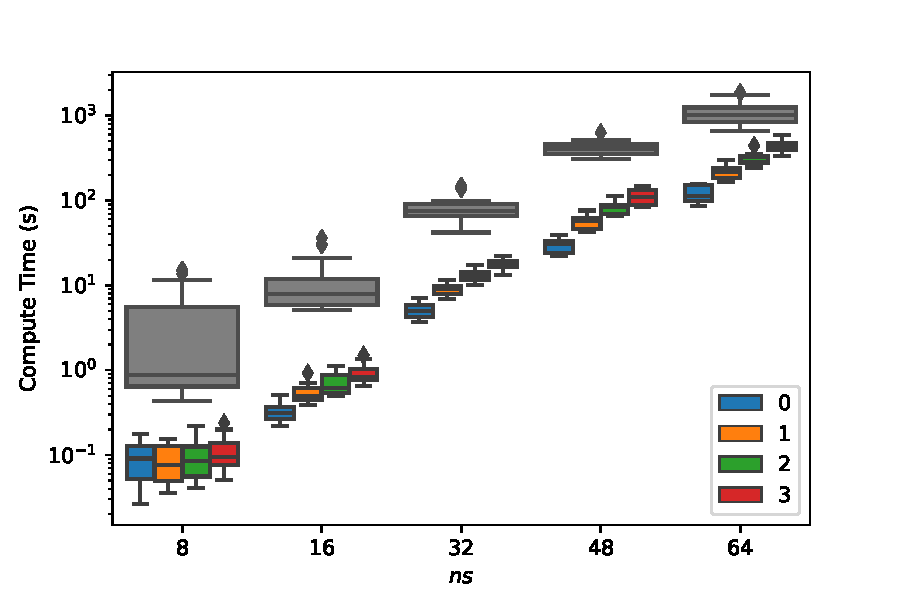
\includegraphics[width=5in]{compute_time_violin}
  \caption{Computation time required for numerical asymptotics and finite difference algorithms over a range of spatial grid sizes using 32 CPUs. Only five grid sizes are shown, with the finite difference and numerical asymptotic algorithm for $n=0,\ldots,3$ terms shown for each grid. The horizontal offset within each grid size is only for visual clarity. TODO: Replace violin plots with box--and--whisker plots.}
  \label{fig:compute_time_violin}
\end{figure}

%Figure \ref{fig:mms_asym_err_time_collapsed} shows the error incurred in the asymptotic approximation versus the computation required for a several values of $b$ and $n$ in order to give a sense of the trade--off between speed and accuracy.
%All calculations are perfomed on the same $64 \times 8$ spatial--angular grid, and errors are compared pointwise to the finite difference calculation using the same value of $b$ on the same grid.
%The dashed black line is a linear fit through the computations in $(\ln\left(\varepsilon/b^n\right), \ln t)$ space with slope $m=0.55 \approx 1/2$.
%This demonstrates the approximate relationship between error, scattering coefficient, and number of terms,
%\begin{equation}
%  \varepsilon t^2 \propto b^n.
%\end{equation}
%So, for example, for a given value of $b$, the error incurred by the scattering coefficient can be halved (for suitable values of $b$), but at the expense of approximately quadrupling the computation time.
%\begin{figure}[H]
%  \centering
%  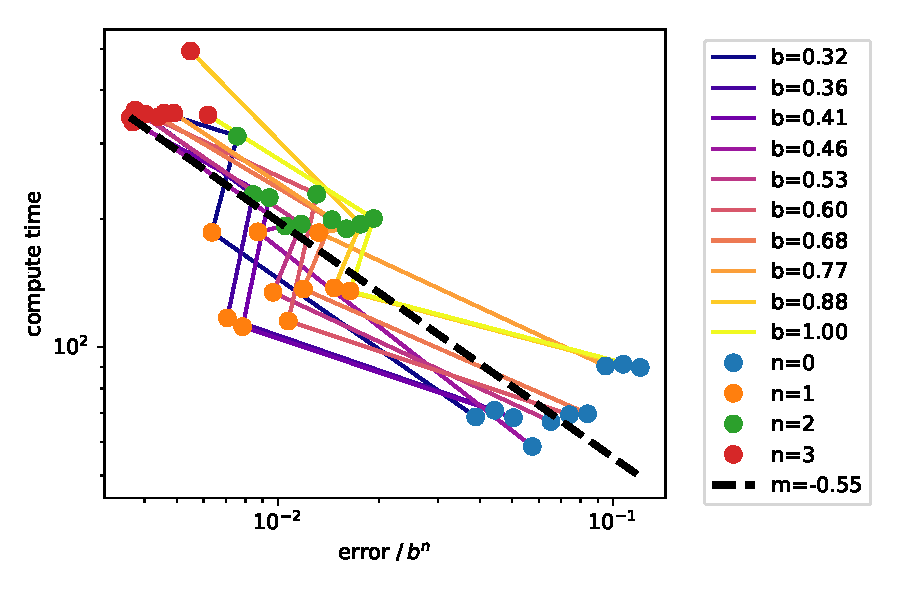
\includegraphics[width=5in]{mms_asym_err_time_collapsed}
%  \caption{To give an idea of the trade--off between accuracy and speed; $n_s=64$, $n_a=8$. . 32 cores.}
%  \label{fig:mms_asym_err_time_collapsed}
%\end{figure}

\subsection{Memory Usage}
Memory usage is perhaps the most important consideration when choosing the algorithm and grid size.
While the numerical asymptotics algorithm requires only a few multiples of the memory required to store the radiance itself, the finite difference algorithm requires the generation and storage of a coefficient matrix several orders of magnitude larger than the solution vector.
These memory requirements are given for a combination of spatial and angular grid sizes in Table \ref{tab:mem_store}.
It is worth noting that using several terms from the asymptotic series does not increase the memory usage, as the same arrays are reused between iterations.

Furthermore, the actual iterative solution of the matrix equation requires the allocation of several multiples of that amount of memory.
A good approximation of the memory required to solve the linear system with GMRES (restarted every 100 iterations) is five times the memory required to store the coefficient matrix.
Even for large grids, the numerical asymptotics approach has not been observed to use more than five gigabytes of memory, which is well within the memory capacity of a common modern laptop or workstation.
On the other hand, the finite difference algorithm uses enormous amounts of memory, from tens of gigabytes for small to medium grids to hundreds of gigabytes for large grids.
These estimates are plotted in Figure \ref{fig:mem_solve}, and listed numerically in Table \ref{tab:mem_solve}.
\begin{figure}[H]
  \centering
  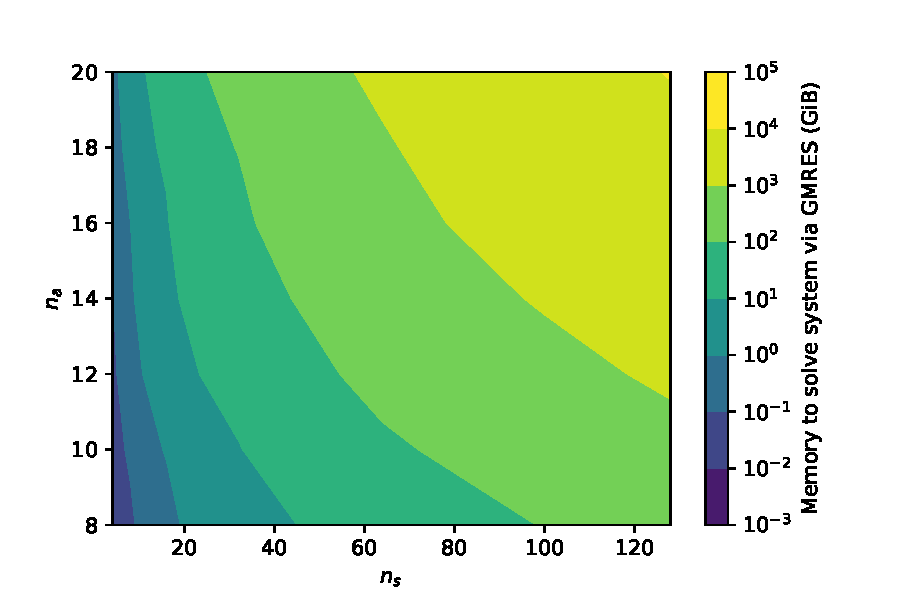
\includegraphics[width=5in]{memory_solve}
  \caption{Estimated memory required to solve the linear system of equations for the finite difference algorithm using GMRES, restarted every 100 iterations. Table \ref{tab:mem_solve} contains the same data in text form.}
  \label{fig:mem_solve}
\end{figure}

\section{Grid Size and Discretization Error}
\label{sec:grid_size}
The size of the spatial--angular grid is an important choice that must be made in order to balance numerical accuracy with computational cost.
Since both the numerical asymptotics and finite difference algorithms are second order methods, the discretization error is prortional to the square of the grid spacing, in both the spatial and angular domains.
In this section, a realistic simulaton is performed on many grids, and the discretization error of each is estimated via Richardson Extrapolation, as described in Section \ref{sec:generalized_re}.
These error estimates allow the spatial and angular components of discretization to be isolated; rules of thumb for both grid spacings are enabled by this analysis.

\subsection{Error Estimatation}
A set of simulations is run for a range of spatial and angular grid sizes with optical properties from Petzold's coastal California waters (HAOCE11), listed in Table \ref{tab:petzold}.
Grid sizes of $n_s=32,48,64,72$ and $n_a=4,8,10,12$ are considered; one simulation is run for every combination of these values.
The average irradiance over the whole domain is calculated for each simulation, which is used as the scalar metric for comparing solutions on disparate grids.
The average irradiances for each simulation are plotted in Figures \ref{fig:gs_avg_irrad_contourf} and \ref{fig:gs_avg_irrad_lines} as functions of the squared grid spacings $ds$ and $da$, given by Equations \eqref{eqn:ds} and \eqref{eqn:da} with $\xmax-\xmin = \ymax-\ymin = \SI{10}{\m}$.
All parameters aside from grid resolution are held constant, so discretization error is the only source of variation within each plot.

\begin{figure}[H]
  \centering
  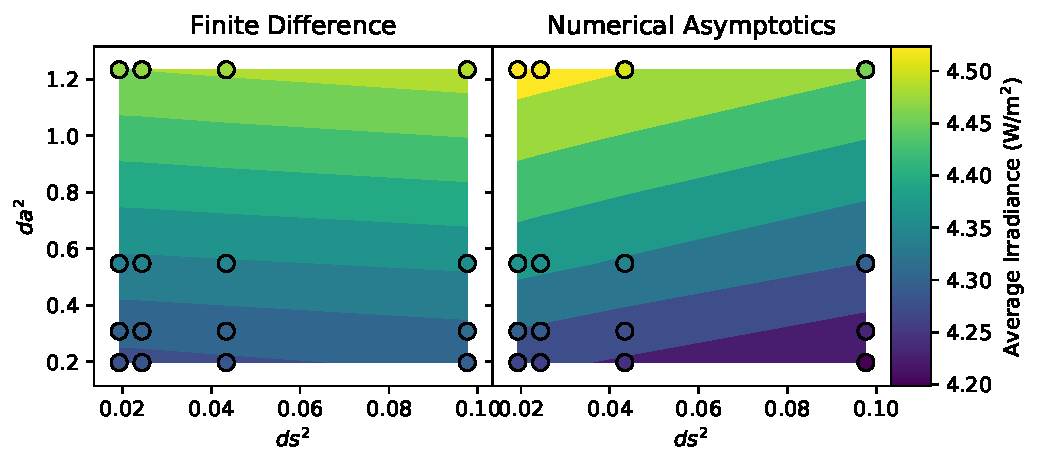
\includegraphics[width=6in]{gs_avg_irrad_contourf}
  \caption{Average irradiance plotted against squared resolution for a variety of grid sizes for finite difference and numerical asymptotics. The linear contours demonstrate that both methods are second order in both resolution parameters.}
  \label{fig:gs_avg_irrad_contourf}
\end{figure}

Notice that in Figure \ref{fig:gs_avg_irrad_lines}, the average irradiance is linear in squared grid spacing for each slice in the resolution space, which 
This pattern holds for both the finite difference and numerical asymptotics algorithms, indicating that all of the grid sizes considered are within the aymptotic region of both methods, since the observed convergence order matches the theoretical order.
This demonstrates that the average irradiance is planar over the whole two--dimensional squared--resolution space, as shown by the parallel linear contours in Figure \ref{fig:gs_avg_irrad_contourf}.


\begin{figure}[H]
  \centering
  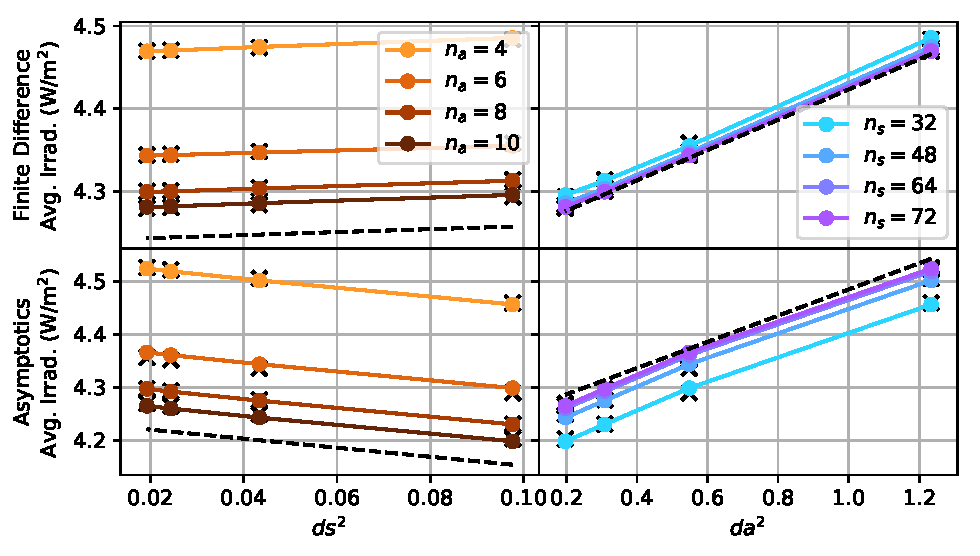
\includegraphics[width=6in]{gs_avg_irrad_lines}
  \caption{Average irradiance plotted against squared resolution. Each line is a one--dimensional projection from Figure \ref{fig:gs_avg_irrad_lines}. Predicted error values are marked with ``x''s, and observed error values with circles. Isolated spatial and angular components of discretization error are plotted with a dashed line on the left and right columns respectively.}
  \label{fig:gs_avg_irrad_lines}
\end{figure}



\subsection{Error Prediction}
The continuum value for the average irradiance is estimated via Richardson extrapolation by fitting a plane through the scalar irradiances in squared--resolution space, as described in Section \ref{sec:generalized_re}.
Values from this plane are shown in Figure \ref{fig:gs_avg_irrad_lines} as ``x''s plotted under the observed errors, shown with circles.
The excellent agreement between the prediction and observation is a testament to the validity of the generalized Richardson eextrapolation method in this circumstance.

By evaluating this plane at $ds=0$, $da=0$, the extrapolated continuum value of average irradiance is found.
The generalized Richardson extrapolation plane is shifted down by the continuum value to construct a model for predict discretization error as a function of grid resolution.
The intersections of this model plane with the $ds=0$ and $da=0$ planes are the isolated angular and spatial components of discretization error respectively.
These isolated components of discretization error are shown in Figure \ref{fig:gs_predicted_err} for both algorithms.
This figure allows for quick estimation of the grid size necessary to achieve a given error threshold.
The total discretization error for a potential grid can be found by taking the sum of the component errors for the algorithm in question.

For example, take the asymptotics algorithm with the grid $n_s=60$, $n_a=20$.
The asymptotics curves are orange, with the dashed line showing the angular component error and the solid line showing the spatial component.
The angular discretization error for this particular grid looks to be about \SI{2e-1}{\W\per\m\squared}, while the spatial discretization error is about \SI{3e-2}{\W\per\m\squared}.
In this case, the spatial grid is unnecessarily fine, since the angular discretization error dominantes by almost an order of magnitude.
In general, the components of grid size should be chosen to produce roughly similar discretization errors so as to avoid unnecessary computation.

From the other perspective, consider an overall target error of $\bar{\varepsilon}=\SI{2e-2}{\W\per\m\squared}$.
This can be achieved by any grid whose spatial and angular error components sum to less than $\bar{\varepsilon}$, but for simplicity, set both component thresholds to $\bar{\varepsilon_s}=\bar{\varepsilon_a}=\SI{1e-2}{\W\per\m\squared}$.
By visual inspection of Figure \ref{fig:gs_predicted_err}, this seems to suggest $n_s=92$, $n_a=22$ for the asymptotics algorithm, or $n_s=42$, $n_a=20$ for the finite difference algorithm.

\begin{figure}[H]
  \centering
  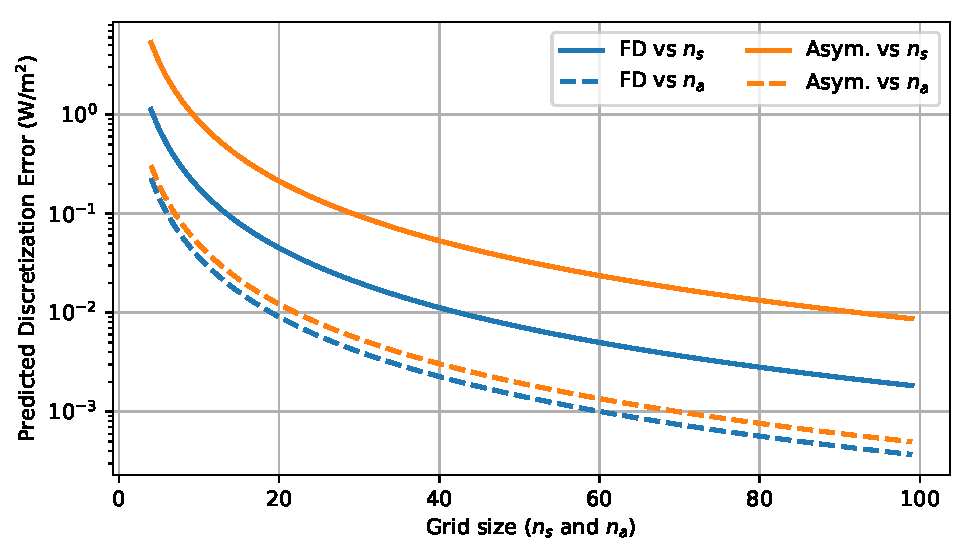
\includegraphics[width=6in]{gs_predicted_err}
  \caption{Predictions for isolated spatial and angular components of discretization error as a function of grid size for both numerical algorithms. Once a target error threshold has been chosen, this figure can be used to estimate the grid sizes that each algorithm would require. The total discretization error is the sum of the spatial and angular parts.}
  \label{fig:gs_predicted_err}
\end{figure}

It is important to note that the error analysis in this section has been performed only for a single set of optical properties (HAOCE11).
Optical properties are sure to have some effect on grid convergence, as they affect the derivatives of the absorption field the solution, thereby impacting the accuracy of quadrature on a particular grid.
Also, keep in mind that $n_a$ ($n_\phi$ in particular) must be an even number, as mentioned in Section \ref{sec:grid}.

\section{Optical Conditions for Asymptotics}
Since the asymptotic approximation is based on a Taylor series expansion around the case of no scattering, it is only valid for relatively small scattering coefficients.
Extremely high--scattering scenarios are out of reach for the asymptotic approximation, and the finite difference approach must be used in those cases.
Whereas in low--scattering waters, adding terms to the asymptotic series tends to decrease the error in the solution, in high--scattering situations, adding terms causes the error to diverge.
Therefore, if the finite difference solution is out of the question for cases of high scattering, the leading order approximation is the best option.
An in--depth analysis of the error incurred by the numerical asymptotics algorithm is presented in this Section.

\subsection{Raw Simulation Results}
\label{sec:iop_study_raw}
In all of the following results, the properties of the kelp are held constant while the optical properties of the water are varied.
Ten values of $a_w$ are taken at equal intervals on a linear scale from \SI{0.1}{\per\m} to \SI{0.5}{\per\m} (inclusive), and ten values of $b$ are taken at even intervals on a log scale from \SI{0.01}{\per\m} to \SI{1.5}{\per\m} (inclusive).
For each set of optical properties, numerical asymptotics is employed with 0, 1, 2, and 3 scattering events, and a finite difference calculation is performed.
A spatial--angular grid size of $72 \times 10$ is used for all calculations.
Each asymptotics calculation is compared to the finite difference calculation with the same optical properties, and a pointwise error is calculated.
Figure \ref{fig:asym_err_vs_b_a01} shows this type of comparison for a single value of $a_w$, varying $b$.
As discussed in Section \ref{sec:num_asym_mms}, the order $n$ approximation converges with roughly order $n+1$.
However, the Figure shows that this trend does not continue indefinitely as $b$ decreases.
This is because although the truncation error is decreasing, the discretization error remains constant.
Therefore, no results with this grid size will show errors below about \SI{0.07}{\W\per\m\squared}.
As a result, simulations with errors below this threshold are discarded in order to gain insight into trends in truncation error.

\newcommand\rdfigwidth{4.5in}

\begin{figure}[H]
  \centering
  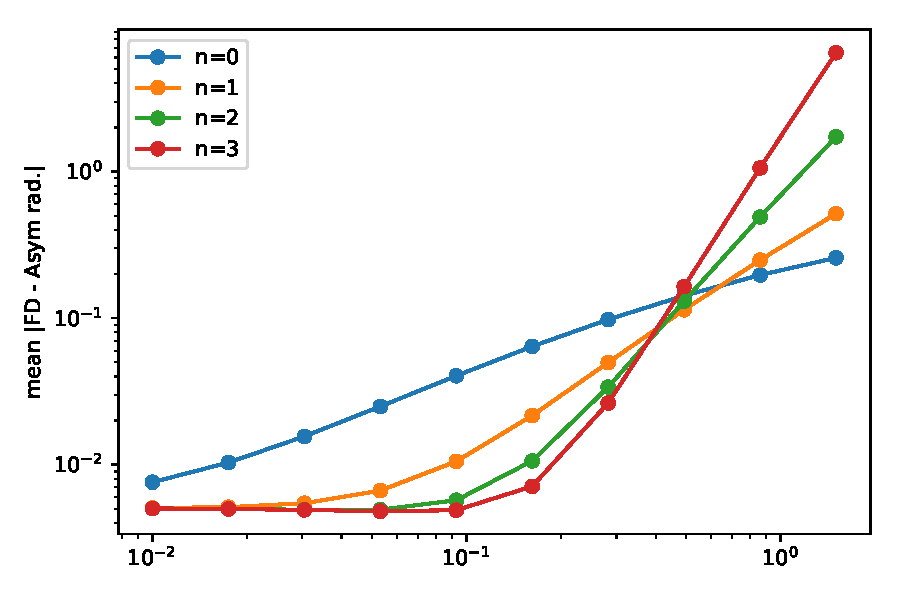
\includegraphics[width=\rdfigwidth]{asym_err_vs_b_a01}
  \caption{Average pointwise difference in irradiance between finite difference and asymptotics solutions for several values of $b$ and $n$ with constant $a=0.1$ in a realistic kelp scenario using a $72\times 10$ grid. Proper convergence of truncation error is observed between $b=0.2$ and $b=0.5$. Below $b=0.2$, discretization error dominates. Above $b=0.5$, the asymptotic series diverges.}
  \label{fig:asym_err_vs_b_a01}
\end{figure}

Figure \ref{fig:asym_err_vs_ab} shows a different slice of the simulation results.
Here, $n=0$ is held constant while $a_w$ and $b$ are plotted on the $x$ and (log) $y$ axes, with average error plotted on the (log) color scale.
Note that mean error does not depend only on $b$.
Rather, errors are largest for waters with low absorption and high scattering, and lowest for low scattering, high absorption.
The clear pattern in the variation of error over the $a_w$--$b$ domain indicates that a third parameter can be calculated sufficiently from $a_w$ and $b$ which is sufficient to determine the accuracy of the approximation.

\begin{figure}[H]
  \centering
  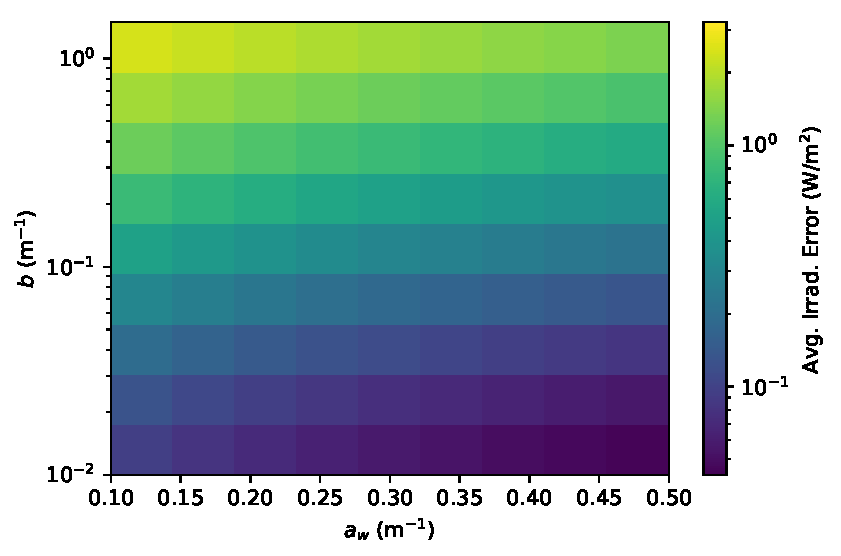
\includegraphics[width=\rdfigwidth]{asym_err_vs_ab}
  \caption{Average pointwise difference in irradiance between finite difference and asymptotics solutions for several values of $b$ and $a$ with constant $n=0$ in a realistic kelp scenario using a $72\times 10$ grid. Note that truncation error is smallest for low--scattering, high--absorption cases, and largest for high--scattering, low absorption.}
  \label{fig:asym_err_vs_ab}
\end{figure}

Figure \ref{fig:best_n_data_vs_ab} shows a similar view of the simulation results as Figure \ref{fig:asym_err_vs_ab}, except that now, the different approximation orders are considered for each set of optical properties, and the order with the lowest error is found.
The order of the best approximation is shown for each case, and the error incurred by that approximation is shown on the color axis.
In the upper left corner, the most difficult cases are shown.
In this region, the zeroth order approximation is most accurate, showing that additional terms cause the solution to diverge.
After a brief transition region, the third order approximation is most accurate, in agreement with Figure \ref{fig:asym_err_vs_b_a01}.

Note that for low scattering, high absorption waters where the error is lowest, the second order approximation seems to perform better than the third order.
As mentioned previously, this is because a lower bound on the total error is imposed by the discretization error, as suggested by Figure \ref{fig:asym_err_vs_b_a01}.
In fact, the second and third order approximations are nearly identical; the former is only slightly better, and no conclusions about truncation error should be drawn from this part of the figure.

\begin{figure}[H]
  \centering
  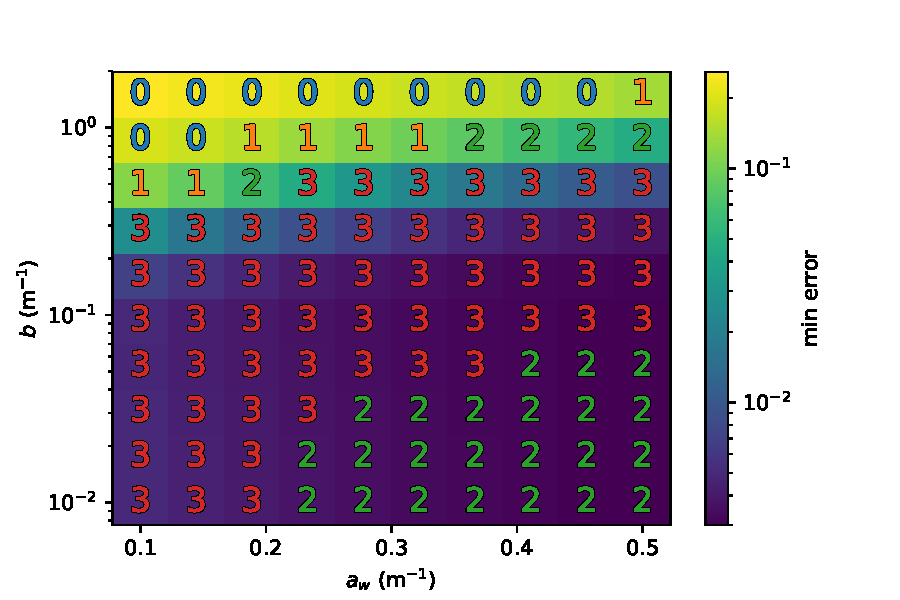
\includegraphics[width=\rdfigwidth]{best_n_data_vs_ab}
  \caption{The best asymptotics solution for each $(a_w,b)$. The value of $n$ used is written in each cell. For high--scattering cases, the $n>0$ terms diverge, so $n=0$ is the best approximation. For most cases, $n=3$ is the best. For very low--scattering cases, discretization error masks the truncation error trend.}
  \label{fig:best_n_data_vs_ab}
\end{figure}

In actual usage, one is concerned not with finding the best approximation, but rather the cheapest one which meets some error threshold.
This concept is explored in Figure \ref{fig:min_n_data_vs_ab}.
TODO: Fix these
In each Figure, an average error threshold of $\bar{\varepsilon}=\SI{0.1}{\W\per\m\squared\per\radian}$, $\bar{\varepsilon}=\SI{0.05}{\W\per\m\squared\per\radian}$, and $\bar{\varepsilon}=\SI{0.01}{\W\per\m\squared\per\radian}$, respectively is set, and the lowest order approximation to meet the error threshold is shown.
The error of that approximation is shown on the color axis.
In each case, there are some optical properties for which the error threshold cannot be met for any $n$.
This is represented by an ``X'' in the figure, and the error of the leading order approximation is shown in color.
Note that as $\bar\varepsilon$ is decreased, the error threshold cannot be satisfied for a larger set of optical properties, and where it is achievable, more scattering terms are required.

\begin{figure}[H]
  \centering
  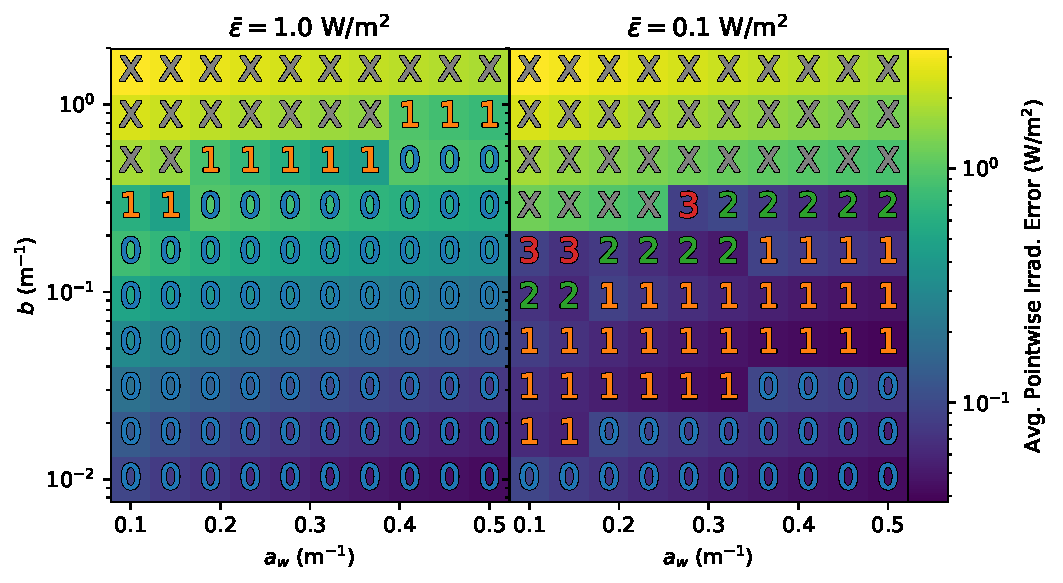
\includegraphics[width=6in]{min_n_data_vs_ab}
  \caption{For each $(a_w,b)$, the smallest value of $n$ which satisfies the error criterion shown above is printed in the cell. ``X'' denotes an optical situation in which the criterion cannot be met since adding further terms makes the solution less accurate, not more. As seen on the left the $n=0$ solution suffices for large error criteria.}
  \label{fig:min_n_data_vs_ab}
\end{figure}

\subsection{Truncation Error Model}
Figure \ref{fig:asym_err_data_xi_model} concisely represents the simulation results for all optical properties and all approximation orders, with error $\varepsilon$ plotted on the vertical axis and $b$ plotted on the color axis.
In the left column, $a_w$ is plotted on the horizontal axis.
On a log--log--log scale, the simplicity of the relationship among these three quantities is striking.
Holding $b$ constant, a log--log linear relationship is apparent between the error $\varepsilon$ and the absorption coefficient $a_w$.
Meanwhile, holding $a_w$ constant, log--uniform increases in $b$ cause log--uniform increases in $\varepsilon$.
That is, $\ln\varepsilon$ seems to increase linearly with $\ln b$ and decrease linearly with $\ln a$.
Restated, it seems that
\begin{equation}
  \varepsilon \propto \frac{b^{c_1}}{a_w^{c_2}}.
\end{equation}

Then, by fitting a plane to the observed values in $(\ln a_w, \ln b, \ln \varepsilon)$ space, a continuous model can be derived for $\varepsilon(a_w, b)$.
Performing this procedure separately for each $n$ value yields values of $c_1$ and $c_2$ which appear to be independent of $n$.
Remarkably, the fit for each order of approximation yields $c_1=3/4$, $c_2=1/2$ to within a few percent variation.
The black ``x''s in Figure \ref{fig:asym_err_data_xi_model} are the predictions of this model, setting $c_1=3/4$ and $c_2=1/2$ explicitly.
Notice how accurately the observed errors are predicted by the model.
This also suggests the definition of a third parameter, as mentioned in Section \ref{sec:iop_study_raw},
\begin{equation}
  \label{eqn:xi}
  \xi = \frac{b^{3/4}}{a_w^{1/2}},
\end{equation}
with the unusual units \SI{}{\m^{-1/4}}.
In the right column of Figure \ref{fig:asym_err_data_xi_model}, $\varepsilon$ is plotted as a function of $\xi$.
Notice that all of the results collapse onto a single line.
Thus, for the sake of understanding the usefulness of the asymptotic series in approximating the true light field, $\xi$ can be used as a single variable to characterize all waters.

\begin{figure}[H]
  \centering
  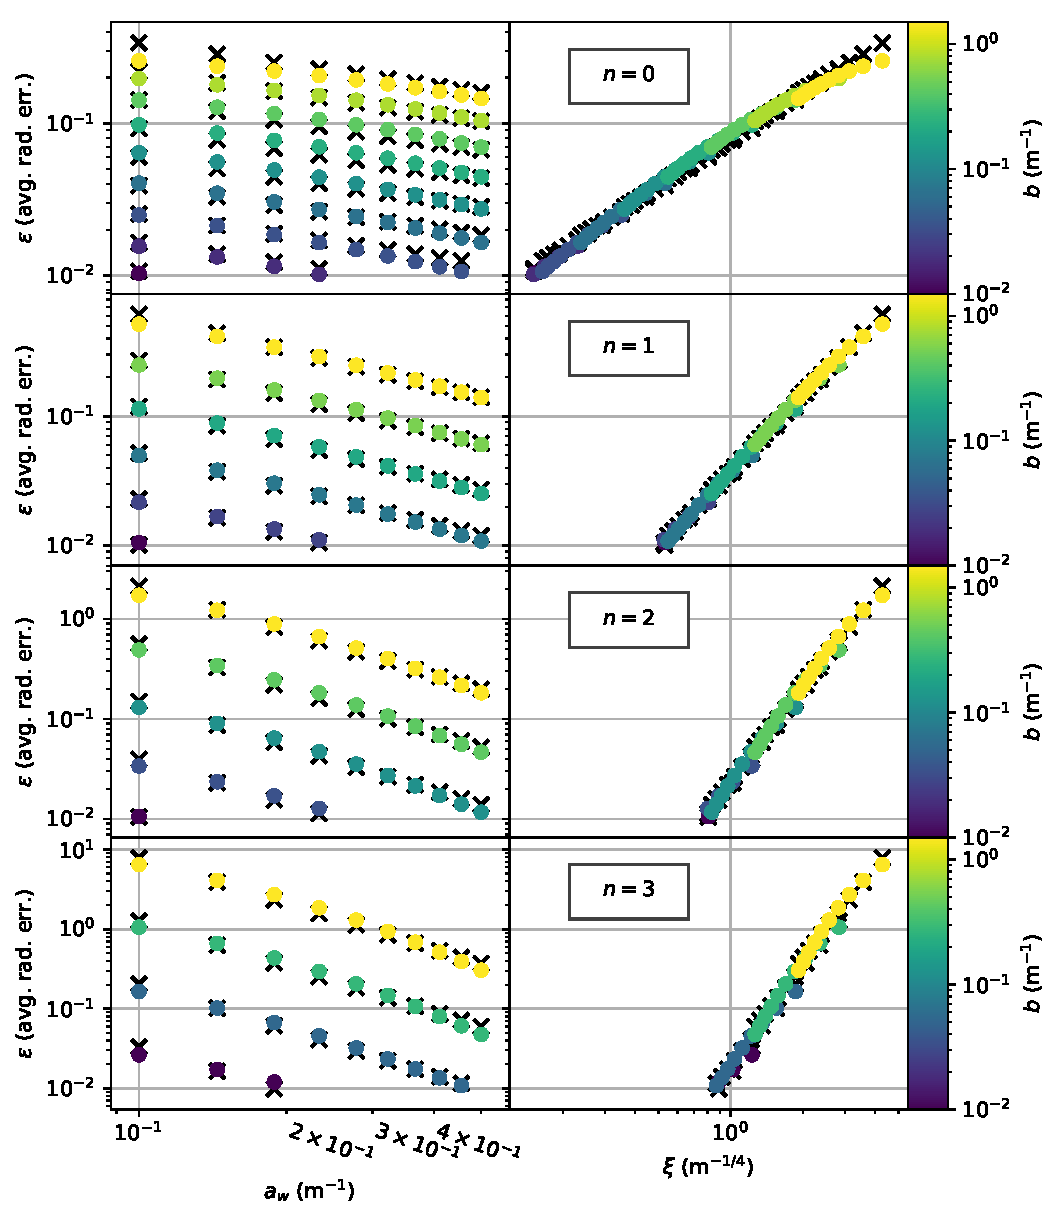
\includegraphics[width=5.5in]{asym_err_data_xi_model}
  \caption{Truncation error plotted against $a_w$ and $\xi$ for each $n$. Simulations dominated by discretization error have been discarded. The right column shows that $\xi$ sufficiently characterizes an optical situation for the sake of predicting truncation error of the asymptotic approximation. Predicted values, marked with ``x''s, are very accurate.}
  \label{fig:asym_err_data_xi_model}
\end{figure}

In Figure \ref{fig:asym_err_vs_xi_all_n_fit_all}, $\varepsilon$ is plotted as a function of $\xi$ for all combinations of $a_w$, $b$, and $n$, effectively combining the right column of Figure \ref{fig:asym_err_data_xi_model} on a single plot.
For each $n$, the log--log plot displays a clear linear relationship, similar to the pattern seen previously in Figures \ref{fig:asym_err_vs_b_a01} and \ref{fig:mms_asym_b_conv}.
However, this figure abstracts that pattern over both $a_w$ and $b$, whereas previously it was seem only for $b$.
Note that the convergence curves for all lines appear to roughly intersect at a characteristic point.
That point, denoted $(\xi^*, \varepsilon^*)$, is significant because it represents a bifurcation in the convergence behavior of the numerical asymptotics algorithm.
For waters with $\xi < \xi^*$, adding terms to the series increases the accuracy of the approximation, whereas for waters with $\xi$ above the threshold value $\xi^*$, adding terms decreases the accuracy.

In order to systematically determine $(\xi^*, \varepsilon^*)$, the log--log convergence curve of order $n+1$ is assumed to have slope $n+1$, which is approximately true, at least for $\xi<\xi^*$.
Further, it is assumed that there is a single point where all of these curves intersect.
This point fully specifies the convergence curves, all other free parameters having been eliminated by the previous assumptions.
Thus, the error for the order $n$ approximation satisfies
\begin{equation}
  \label{eqn:ln_eps_n}
  \ln\left(\varepsilon_n(\xi)\right) - \ln\varepsilon^* = (n+1)\left(\ln\xi - \ln\xi^*\right),
\end{equation}
or equivalently,
\begin{equation}
  \label{eqn:eps_n}
  \varepsilon_n(\xi) = \varepsilon^* \left(\frac{\xi}{\xi^*}\right)^{n+1}.
\end{equation}

Then, a residual function is constructed which accumulates squared differences between the fit functions and their corresponding data points, weighting all squared errors by $1/\varepsilon$ in order to deem the runs with lower errors more important since errors diverge for large $\xi$ values and do not fit the linear function quite as well.
A numerical optimization algorithm is then used to search the two dimensional parameter space for the minimizers of the residual, which produces the point $(\xi^*, \varepsilon^*)$.
This procedure yields the result
\begin{align}
  \xi^* &= \SI{1.58}{\m^{-1/4}}, \\
  \varepsilon^* &= \SI{1.30}{\W\per\m\squared},
\end{align}
as shown in Figure \ref{fig:asym_err_vs_xi_all_n_fit_all}.
Thus, waters characterized below this threshold are worth considering for solution via numerical asymptotics, whereas others are better suited for a finite difference solution.

\begin{figure}[H]
  \centering
  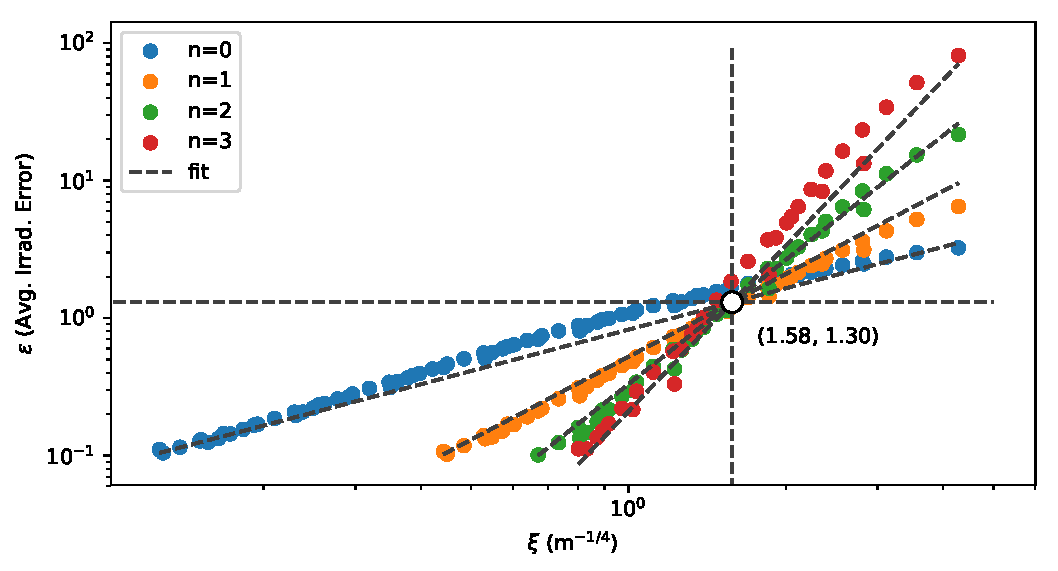
\includegraphics[width=6in]{asym_err_vs_xi_all_n_fit_all}
  \caption{All data from the right column of \ref{fig:asym_err_data_xi_model} on a single plot demonstrates a characteristic $\xi=\xi^*$ above which the asymptotic series diverges. This observation permits a simple model for predicting truncation error.}
  \label{fig:asym_err_vs_xi_all_n_fit_all}
\end{figure}

The determination of $\xi^*$ and $\varepsilon^*$ marks the construction of a simple analytical model given by Equation \eqref{eqn:eps_n} which predicts the errors for any set of aquatic optical properties.
Figure \ref{fig:asym_err_model_vs_ab_all_n} shows the predictions of this model for several values of $a_w$, $b$, and $n$, with $\varepsilon$ plotted on the color axis.
Note that $\xi^*$ is a contour in $(a_w, b)$ space, and is marked on the figure with a dashed white line.
$\xi<\xi^*$ is the region to the lower right of the threshold, and $\xi>\xi^*$ is the region to the upper left.
Also keep in mind that this model and its predictions deal only with truncation error, and that discretization error distorts the actual solution accuracy, as seen in Figures \ref{fig:asym_err_vs_b_a01} and \ref{fig:best_n_data_vs_ab}.

\begin{figure}[H]
  \centering
  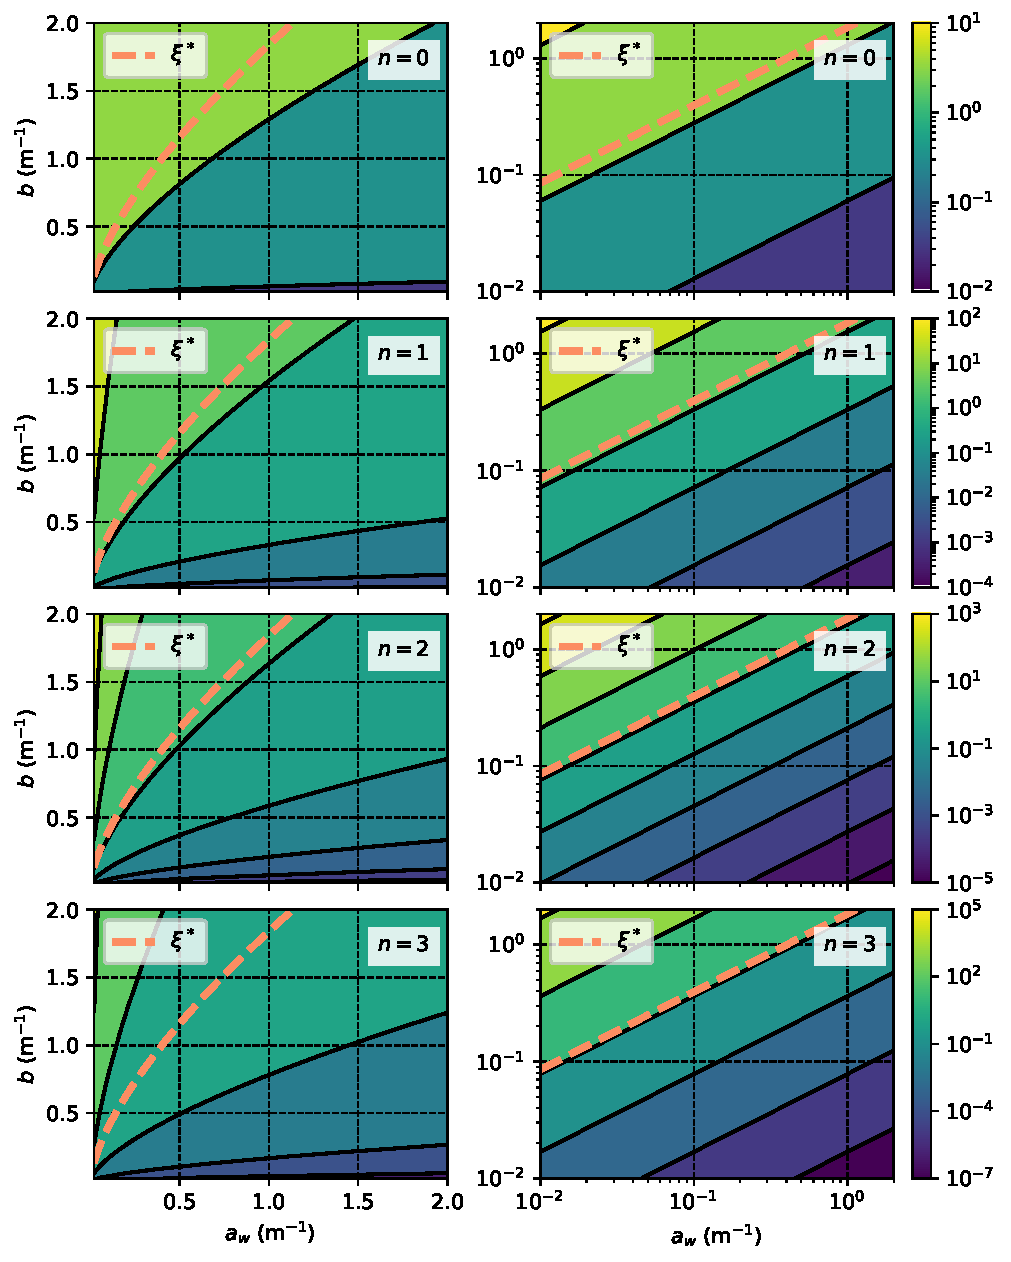
\includegraphics[width=5.75in]{asym_err_model_vs_ab_all_n}
  \caption{Predicted truncation error for a range of $a_w$ and $b$ values. $n$ varies over plot rows. Linear--linear scale on the left, log--log scale on the right. The asymptotic series converges only for $(a_w,b)$ values to the right of the $\xi^*$ contour.}
  \label{fig:asym_err_model_vs_ab_all_n}
\end{figure}

This model can now be used to produce general guidelines for the choice of $n$ given a desired error.
Assuming that a maximum error $\varepsilon=\bar\varepsilon$ is permissible, the minimum order of $n$ which produces $\varepsilon$ is desired.
This order, denoted $\bar{n}$, can determined by solving Equation \eqref{eqn:ln_eps_n} for $n$ when $\varepsilon=\bar{\varepsilon}$ and rounding up to the nearest integer.
That is,
\begin{equation*}
  \bar{n} = \ceil\left(\frac{\ln\bar{\varepsilon} - \ln\varepsilon^*}{\ln\xi - \ln\xi^*} - 1 \right),
\end{equation*}
which is equivalent almost everywhere to
\begin{equation}
  \label{eqn:n_bar}
  \bar{n} = \floor\left(\frac{\ln\bar{\varepsilon} - \ln\varepsilon^*}{\ln\xi - \ln\xi^*}\right).
\end{equation}

Figure \ref{fig:nbar_model_vs_ab_3eps} shows $\bar{n}$ up to $\bar{n}=3$ for $\bar{\varepsilon}=0.1$, $\bar{\varepsilon}=0.05$, and $\bar{\varepsilon}=0.01$.
The $\xi^*$ contour is plotted.
Assuming that $\bar{\varepsilon}<\varepsilon^*$, if higher contours of $\bar{n}$ were plotted, they would approach the $\xi^*$ contour as $\bar{n} \to \infty$ since no accuracy better than $\varepsilon^*$ is achievable by any order approximation when $\xi > \xi^*$.

To summarize this analysis, once an error threshold $\bar{\varepsilon}$ is chosen, the optical properties $a_w$ and $b$ determine the optimal numerical approach according to Figure \ref{fig:nbar_model_vs_ab_3eps} and Equation \eqref{eqn:n_bar}.
If $\xi^*(a_w, b) > \xi^*$, then the finite difference algorithm should be used if possible.
If memory or computation time requires the numerical asymptotics algorithm to be used, then the $n=0$ approximation should be used, effectively ignoring scattering.

If $\bar{n}>3$ (i.e., the gray region between $\xi^*$ and $\bar{n}=3$), it is theoretically possible to achieve the desired accuracy in this region by continuing to add terms, however, this is not recommended since the closer $\xi$ is to $\xi^*$, the more likely it is that higher order terms will cause the solution to diverge due to some unexpected deviation in the actual performance of the algorithm from the theoretical error model presented here.
As a compromise, $n=2$ or $n=3$ could be used in this region to balance the severity of divergence in the case of failure with the improved accuracy of the solution in the case of successful convergence.
Finally, in any of the easier regions defined by $\bar{n} \leq 3$, the optimal trade--off between accuracy and computation time is achieved by using $n=\bar{n}(a_w, b)$.

\begin{figure}[H]
  \centering
  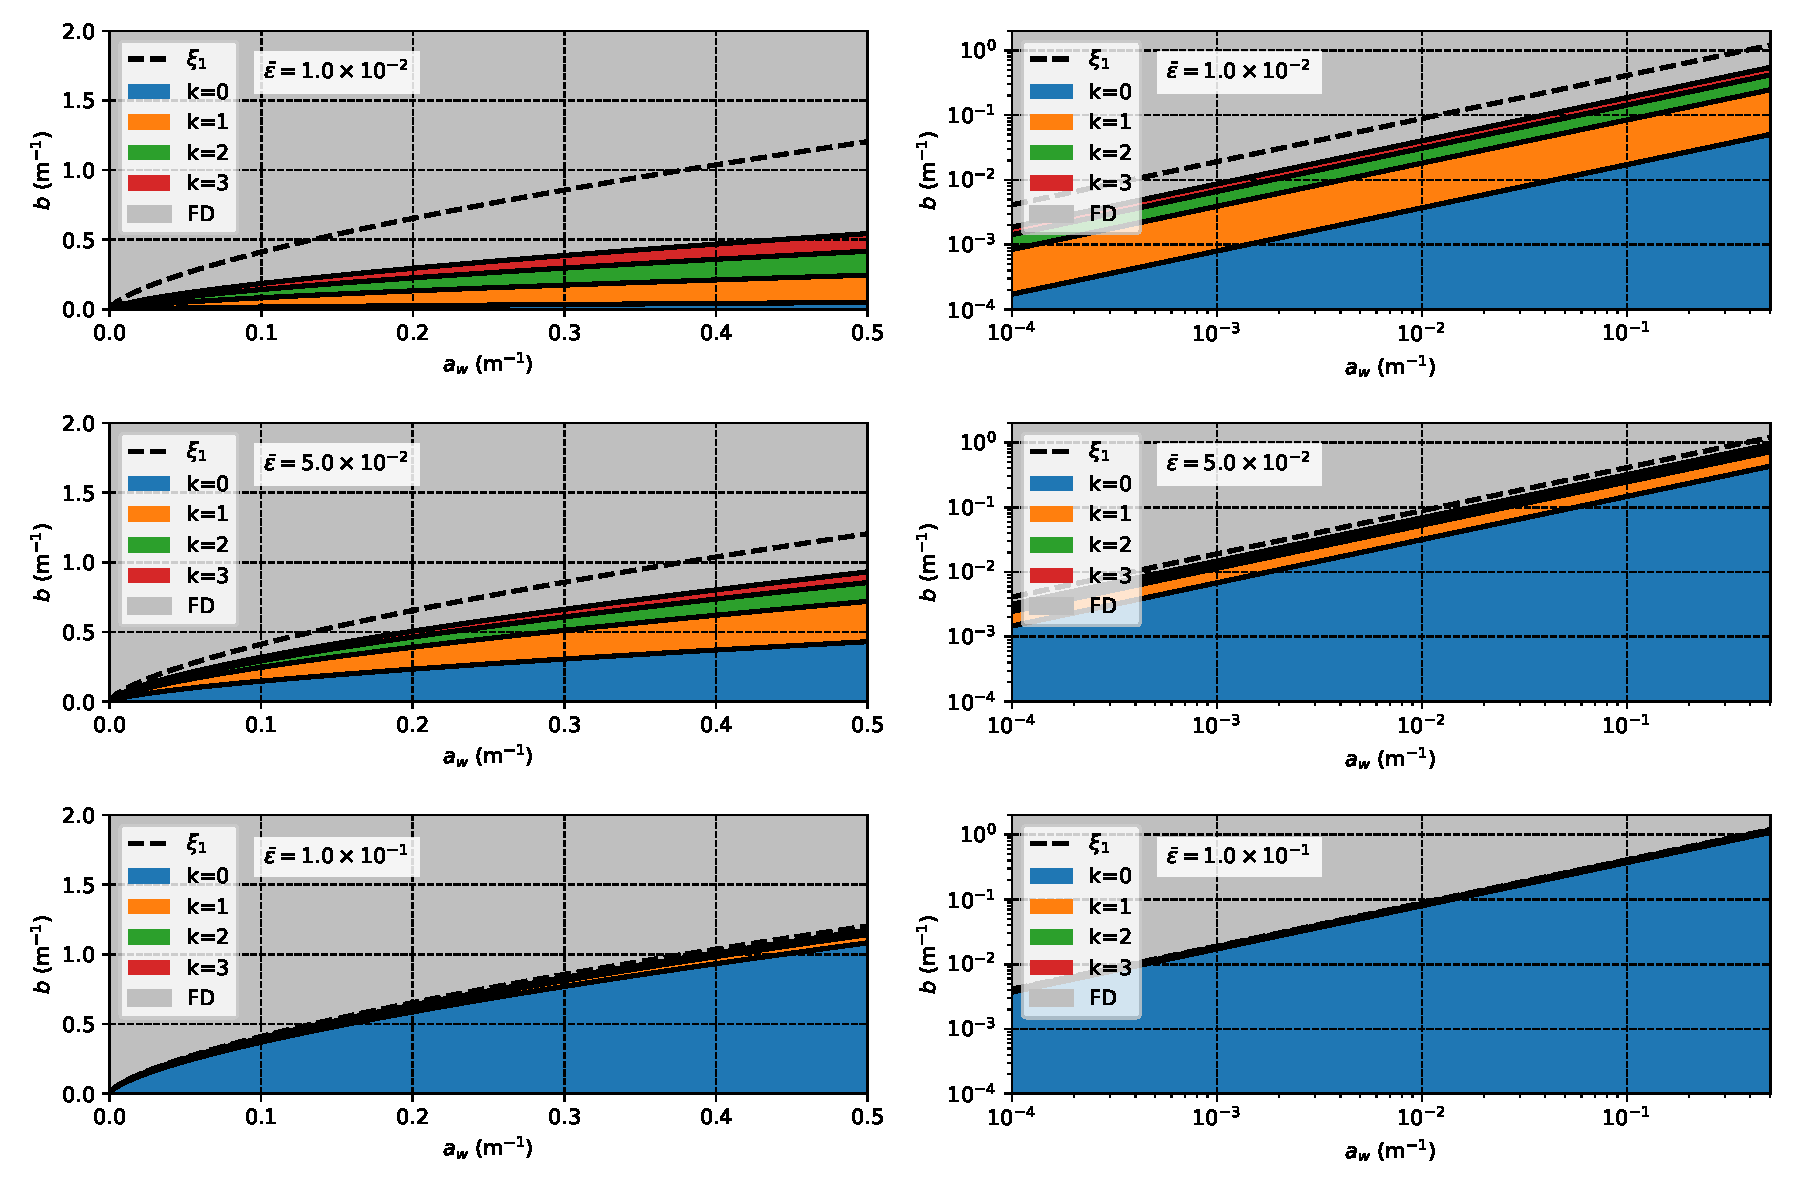
\includegraphics[width=5.5in]{nbar_model_vs_ab_3eps}
  \caption{Recommended $n=\bar{n}$ value as a function of $(a_w,b)$ to achieve the truncation error criteria $\bar{\varepsilon}=0.1,0.5,1.0\SI{}{W\per\m\squared}$ for the three plot rows.}
  \label{fig:nbar_model_vs_ab_3eps}
\end{figure}


\section{Comparison to Other Light Models}

Now that recommendations have been given for the choice of solution method, with the computational cost and accuracy of each having been discussed, all that remains is to compare the solutions obtained from the model presented in this thesis to other available models for the light field.
Two simple models are used; in both cases, the number of calculations can be counted on two hands, whereas the model of this thesis involves many millions of calculations.
Whether the insight gained from the more complex model is worth the computational expense depends on the purpose of the calculation, and is a decision for the reader to make according to their best judgment for the situation.

\subsection{Simpler Models}
The first model is the simplest conceivable light model --- exponential attenuation with a constant absorption coefficient $a=a_w$.
That is, the simplest solution is to ignore the kelp entirely.
Of course, a depth--dependent absorption coefficient is likely to be used in a real simulation, but for the sake of the comparison, a constant $a_w$ is used.
The irradiance in this case is simply
\begin{equation}
  I(z) = \exp\left(-a_w z \right).
\end{equation}

The second light model, presented in \citep{broch_modelling_2012}, accounts for the kelp by adding a depth--dependent term to the absorption coefficient related to the area and spatial density of the seaweed.
The model is described by
\begin{align}
  \frac{dI}{dz} &= -\left(a_w + k_{\mbox{kelp}}(z)\right),
  \label{eqn:exp_kelp_dIdz}\\
  k_{\mbox{kelp}}(z) &= -\ln(1-A_k(1-(1-AD)^{\rho_f(z)})),
  \label{eqn:exp_kelp_k}
\end{align}
where $A_k$ is the kelp absorptance, $D$ is the number of vertical kelp ropes per horizontal \SI{}{\m\squared}, $A(z)$ is the average area of the kelp fronds per meter vertical rope, and $\rho_f$ is the number of kelp fronds per vertical meter of rope.
Then,
\begin{equation}
  D = \frac{1}{\left(\xmax-\xmin\right) \left(\ymax-\ymin\right)},
\end{equation}
and the mean frond $A$ is calculated from the mean frond length according to Equation \eqref{eqn:area_from_length} as
\begin{equation}
  A = \frac{{\mu_l}^2}{2f_r}.
\end{equation}

Once $k_{\mbox{kelp}}(z)$ is calculated according to Equation \eqref{eqn:exp_kelp_k}, then the solution of Equation \eqref{eqn:exp_kelp_dIdz} is a simplified version of Equation \eqref{eqn:asymptotics_ode_0} with $\tilde{a}(z)=a_w+k_{\mbox{kelp}}(z)$ and $\tilde{\sigma}_0=0$.
The solution is therefore the analogous simplification of Equation \eqref{eqn:asymptotics_soln_0}, namely
\begin{equation}
  I(z) = I_0 \exp\left(-a_wz - \int_0^z k_{\mbox{kelp}}(z')\, dz' \right).
\end{equation}

\subsection{Comparison Results}
In Figure \ref{fig:compare_models_haoce11_both}, the light model of this thesis is compared to simpler models under the conditions described in Section \ref{sec:standalone_context}.
In the figures, the first model described in this Chapter, which ignores the kelp entirely, is plotted with a black dashed line.
The second model, which uses an additional term in the absorption coefficient to describe the kelp, is plotted with a dashed blue line.
The no--scattering numerical asymptotics solution is plotted in solid red.
Since the above two models do not consider scattering, both the finite difference and asymptotic solutions are plotted for a range of $b$ values, with the finite difference $b$ described by the left color bar, and the asymptotic $b$ described by the right color bar, so as to distinguish between the two sets of curves.

In each of the three Figures, a different value of $n$ is used for the asymptotic approximations for $b>0$: $n=1$, $n=2$, and $n=3$ for Figure \ref{fig:compare_models_haoce11_both}.
In the left column of each figure, the average irradiance is plotted as a function of depth for each of the calculations from the light model of this thesis, calculated over the entire horizontal domain.
In the right column, the perceived irradiance, as described in Section \ref{sec:perceived_irrad}, is shown for the asymptotics and finite difference calculations.

First, note that the no--kelp model predicts the highest light levels throughout the domain, as should be expected since it ignores a significant aspect of the light reduction.
The simple kelp model agrees with the no--kelp model at the surface, but then reduces more quickly once the kelp, which is largest at $z=2$, is introduced.
At the bottom of the domain where there is little kelp remaining, the two curves are seen to be parallel in the log--linear scale, showing that the absorption coefficients are equal as at the surface.
Looking at the left column, the average irradiance from no--scattering solution to the 3D model appears to agree quite well with the simple kelp model, especially near the surface and bottom, where both models are approximately reduced to the first model.
In the $z=2$ region where the most kelp is present, the 3D model predicts higher absorption than the simpler 1D model.
However, between $z=3$ and $z=4$, the 3D kelp model decreases more slowly than the 1D model, perhaps because light is able to penetrate the water in regions where the kelp is not present, and the multitude of angles in which the light travels allow some of the rays to reach even the lower depths without being absorbed by the kelp.

As for the right column, the perceived irradiance is clearly much lower than the average irradiance and the other models.
This makes sense, as the light is dimmest in the regions of highest kelp density, and the perceived irradiance weights these regions the highest, practically ignoring the edges of the domain where light is absorbed only by the water; these regions skew the average irradiance upward although they are not actually representative of the light field where photosynthesis is occurring.
From this point of view, it seems that the other two light models significantly overestimate the amount of light available where it actually matters.

Considering the finite difference solution, the most visible effect of increasing scattering is to decrease the light field towards the bottom of the domain.
Of course, scattering does not cause that light to be lost entirely.
Rather, it tends to reflect it towards the surface, where increases in scattering lead to higher light levels.
This is noteworthy since the light available very close to the surface is significantly higher than it is a few meters below.
This tendency for scattering to insulate the upper region of the water may prove to be important in understanding how photosynthesis near the ocean's surface differs from photosynthesis at greater depths.

\begin{figure}[H]
  \centering
  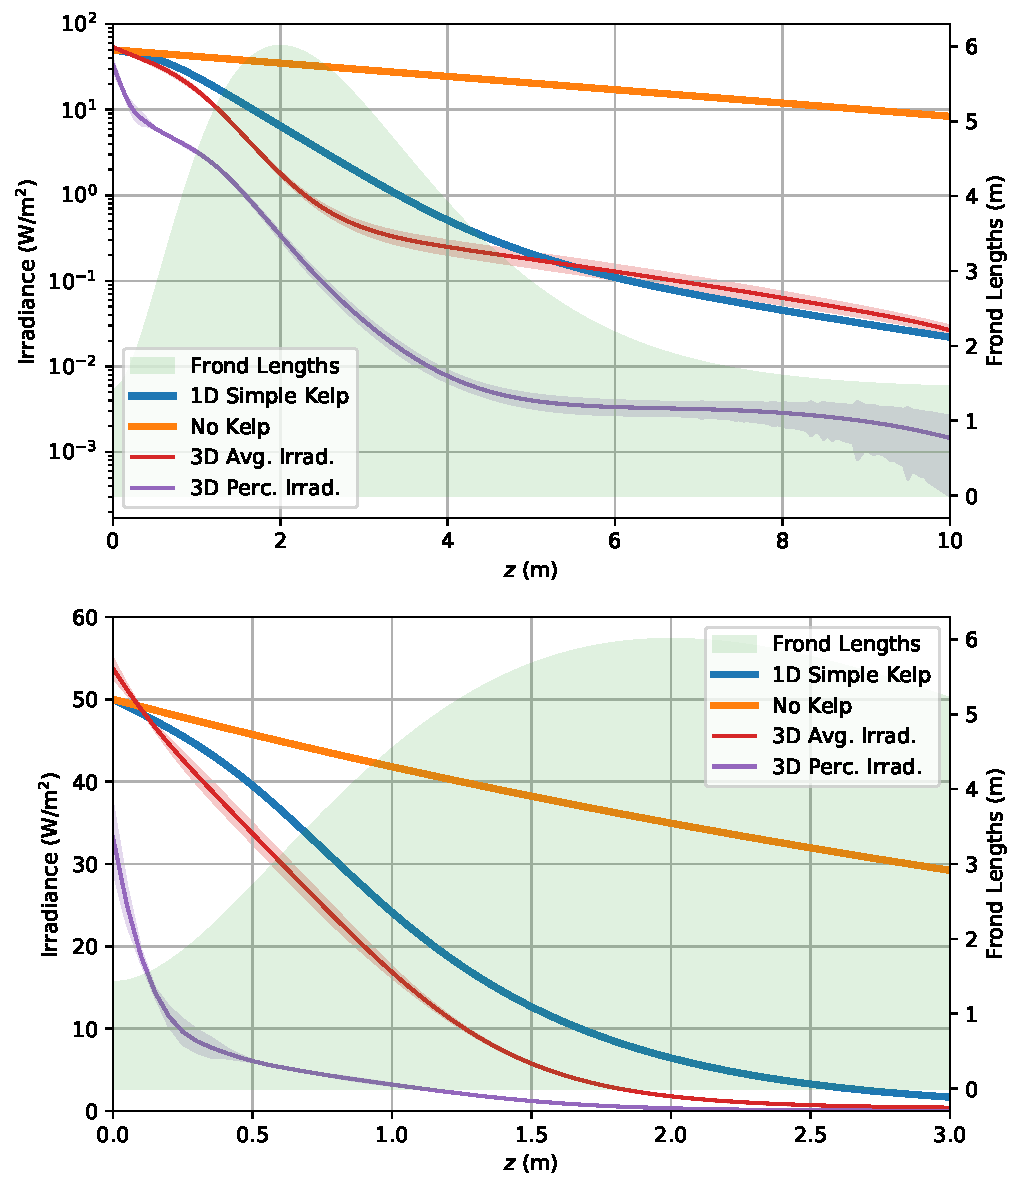
\includegraphics[width=6in]{compare_models_haoce11_both}
  \caption{Average irradiance and perceived irradiance from finite difference compared to simpler light models for the case of coastal California water (HAOCE11) with realistic kelp growth. Frond lengths over depth are shown on the right--hand axis. Discretization error is shown by error bands for perc. irrad. and avg. irrad.}
  \label{fig:compare_models_haoce11_both}
\end{figure}


\begin{figure}[H]
  \centering
  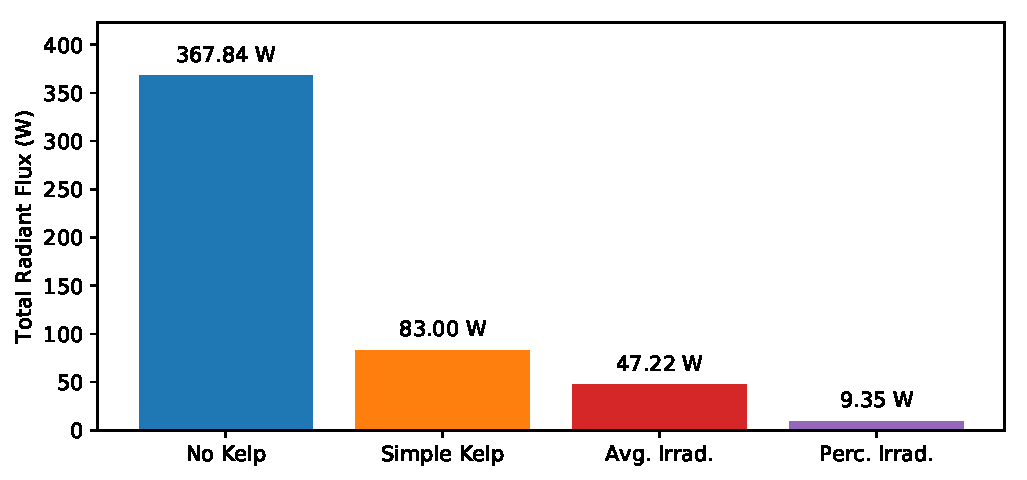
\includegraphics[width=6in]{compare_models_haoce11_flux}
  \caption{Total radiant flux in Watts through kelp predicted by each model.}
  \label{fig:compare_models_haoce11_flux}
\end{figure}
